% =======================================================================
% Semantics
% =======================================================================

\section{Semantics}
\begin{frame}[fragile]{Match semantics}
    Assarin et al.

    \textit{The automaton for \underline{$[\![a]\!]$}}, $a\in\Sigma$ is $(\{s,f\},\emptyset,\Delta,\Sigma,s,\{f\})$ where the transition relation is $\Delta={(s,true,\emptyset,a,f)}$.
    
    \begin{lstlisting}[language=c++,basicstyle=\small]
void Visit(Match match)
{
    TimedAutomaton ta = new(_regex);
    
    State initial = ta.AddState(newInitial: true);
    State final = ta.AddState(true);

    ta.AddEdge(initial, final, match.Token.Match);

    _stack.Push(ta);
}
    \end{lstlisting}
\end{frame}

\begin{frame}{Union semantics}
    Assarin et al.

    \textit{The automaton for $[[\varphi_1\vee\varphi_2]]$ is $(Q_1\cup Q_2 \cup \{s\},C_1\cup C_2,\Delta,\Sigma,s,F_1\cup F_2)$, where $\Delta$ is constructed
by adding to $\Delta_1\cup \Delta_2$ two new $\epsilon$-transitions $(s, x = 0,\emptyset,\epsilon,s_i)$, where $x$ is any clock and $i\in{1,2}$
(if there is no clock in the automata we should add one).}

\usetikzlibrary {automata,positioning}
% "A|B"
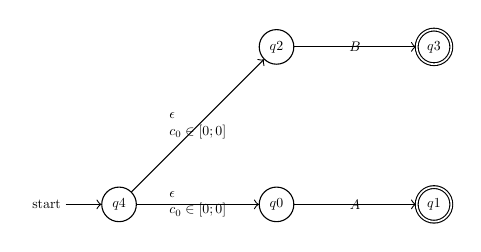
\begin{tikzpicture}[every node/.style={scale=0.5}]
    \node[state] at (2, 0)(q0){$q0$};
    \node[state, accepting] at (4, 0)(q1){$q1$};
    \node[state] at (2, 2)(q2){$q2$};
    \node[state, accepting] at (4, 2)(q3){$q3$};
    \node[state, initial] at (0, 0)(q4){$q4$};
    
    \path[->]
        (q0)edge node[align=left]{$A$}(q1)
        (q2)edge node[align=left]{$B$}(q3)
        (q4)edge node[align=left]{$\epsilon$\\$c_0\in[0;0]$}(q0)
        (q4)edge node[align=left]{$\epsilon$\\$c_0\in[0;0]$}(q2)
        ;
\end{tikzpicture}

% "A|B"
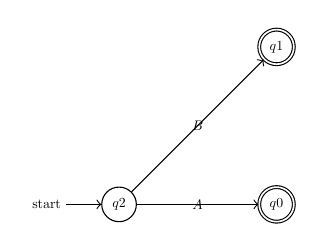
\begin{tikzpicture}[every node/.style={scale=0.5}]
    \node[state, accepting] at (2, 0)(q0){$q0$};
    \node[state, accepting] at (2, 2)(q1){$q1$};
    \node[state, initial] at (0, 0)(q2){$q2$};
    
    \path[->]
        (q2)edge node[align=left]{$A$}(q0)
        (q2)edge node[align=left]{$B$}(q1)
        ;
\end{tikzpicture}
\end{frame}

\begin{frame}{Union semantics revised}
    % We can improve upon union by removing unnecessary epsilon transitions.
\begin{definition}
    Union\label{def:union-semantics}
    
    \sembox{
        $\semaut{\varphi_1|\varphi_2}=
        \left\{\begin{array}{ll}
            \semaut{(\epsilon\cdot\varphi_1)\cup\varphi_2} & if (q_1,\phi_1,p_1,a,s_1)\in\Delta_1 \\
            \semaut{\varphi_1\cup(\epsilon\cdot\varphi_2)} & if (q_2,\phi_2,p_2,a,s_2)\in\Delta_2 \\
            \automaton & otherwise \\
        \end{array}\right.
        $
        
        Where
        
        $f\transition=
        \left\{\begin{array}{ll}
            \transition[][s] & if q\in\{s_1,s_2\} \\
            \transition & otherwise \\
        \end{array}\right.
        $
        
        $Q=Q_1\cup Q_2 \cup {s}\backslash\{s_1,s_2\}$
        
        $C=C_1\cup C_2$
        
        $\Delta=f(\Delta_1\cup\Delta_2)$
        
        $F=F_1\cup F_2\backslash\{s_1,s_2\}$
    }
\end{definition}
\end{frame}

\begin{frame}[fragile]{Union implementation}
    \begin{lstlisting}[language=c++,basicstyle=\tiny]
(TimedAutomaton right, TimedAutomaton left) = (_stack.Pop(), _stack.Pop());
EpsilonConcat(right);
EpsilonConcat(left);
TimedAutomaton ta = new(left, right, e => IsNotInitial(e.From), IsNotInitial);

State initial = ta.AddState(newInitial: true);

foreach (Edge edges in left.GetEdgesFrom(left.InitialState!)
    .Concat(right.GetEdgesFrom(right.InitialState!)))
{
    Edge e = ta.AddEdge(initial, edges.To, edges.Symbol);
    e.AddClockRanges(edges.GetClockRanges());
    e.AddClockResets(edges.GetClockResets());
}

static void EpsilonConcat(TimedAutomaton ta)
{
    if (ta.GetEdgesTo(ta.InitialState!).Any())
    {
        State oldInitial = ta.InitialState!;
        State newInitial = ta.AddState(ta.IsFinal(oldInitial), true);
        Edge edge = ta.AddEdge(newInitial, oldInitial, "\0");
    }
}
    \end{lstlisting}
\end{frame}

\begin{frame}[fragile]{Lazy intersection}
    Lazily generate new states
    \begin{lstlisting}[basicstyle=\tiny]
State GetNewState(State lState, State rState)
{
    if (!newLocs.TryGetValue((lState, rState), out State? state))
    {
        state = ta.AddState();
        newLocs[(lState, rState)] = state;
    }

    return state;
}
    \end{lstlisting}
\end{frame}

% =======================================================================
% Timed word generator
% =======================================================================
\section{Timed words}
\begin{frame}[fragile]{Timed word generation}
    \begin{columns}
        \begin{column}{0.5\textwidth}
            nasa.gov
            \begin{lstlisting}[basicstyle=\tiny]
00 00 00 04 CDR
Roger. Clock.

00 00 00 13 CDR
Roger. We got a roll program.

00 00 00 15 CMP
Roger. Roll.

00 00 00 34 CDR
Roll's complete and the pitch is programed.

00 00 00 44 CDR
One Bravo.

00 00 01 02 CC
Apollo 11, Houston. You're good at 1 minute.
...
            \end{lstlisting}
        \end{column}
        \begin{column}{0.5\textwidth}
            apollo11transcript.csv
            \begin{lstlisting}[basicstyle=\tiny]
CDR, 4


CDR, 13


CMP, 15


CDR, 34


CDR, 44


CC, 62

...
            \end{lstlisting}
        \end{column}
    \end{columns}
\end{frame}

\begin{frame}[fragile]{Words as timed automata.}
    In Uppaal
    \begin{columns}
        \begin{column}{0.5\textwidth}
            % "(<CDR>|<CC>|<CMP>)+"
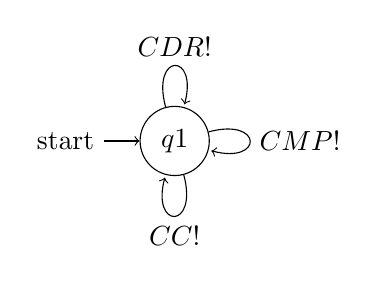
\begin{tikzpicture}[auto]
    \node[state, initial] at (0, 0)(q1){$q1$};
    
    \path[->]
        (q1)edge [loop above] node[align=left]{$CDR!$}(q1)
        (q1)edge [loop below] node[align=left]{$CC!$}(q1)
        (q1)edge [loop right] node[align=left]{$CMP!$}(q1)
        ;
\end{tikzpicture}
            
        \end{column}
        \begin{column}{0.5\textwidth}
            \begin{lstlisting}[basicstyle=\tiny]
update: index++
guard: index <= 8439 &&
    word[index] == "CDR" &&
    times[index] == c0
            \end{lstlisting}
        \end{column}
    \end{columns}
    \begin{lstlisting}[basicstyle=\tiny]
clock c0;
int32_t index = 0;
const string word[8439] = {"CDR", "CDR", "CMP", "CDR", "CDR", "CC", ... }
clock_t times[8439] = {4, 13, 15, 34, 44, 62, ... }
    \end{lstlisting}
\end{frame}

% =======================================================================
% Pruning
% =======================================================================
\section{Pruning}
\begin{frame}{Example}
    $$C(A[5;10]\&(BA|A)[1;3])$$
    % Generated by: TimedRegex, Version = 1.0.0.0
% Date 5/14/2024 6:44:16 PM
\usetikzlibrary {automata,positioning}
\scalebox{0.9}{
    % "C(A[5;10]&(BA|A)[1;3])"
    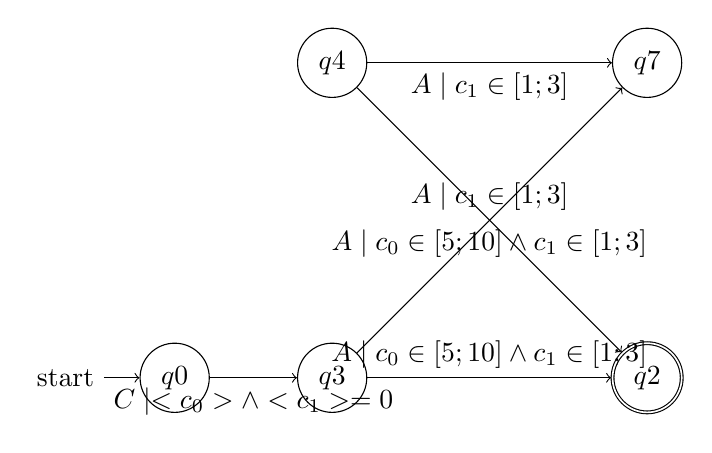
\begin{tikzpicture}[auto]
        \node[state, initial] at (0, 0)(q0){$q0$};
        \node[state] at (2, 0)(q3){$q3$};
        \node[state] at (2, 4)(q4){$q4$};
        \node[state] at (6, 4)(q7){$q7$};
        \node[state, accepting] at (6, 0)(q2){$q2$};
        
        \path[->]
            (q4)edge node[below]{$A\mid c_1\in[1;3]$}(q7)
            (q3)edge node[above]{$A\mid c_1\in[1;3]$}(q7)
            (q4)edge node[below]{$A\mid c_0\in[5;10]\wedge c_1\in[1;3]$}(q2)
            (q3)edge node[above]{$A\mid c_0\in[5;10]\wedge c_1\in[1;3]$}(q2)
            (q0)edge node[below]{$C\mid <c_0>\wedge<c_1>=0$}(q3)
            ;
    \end{tikzpicture}
}

\captionof{figure}{Lightly pruned automaton, to be used as an example.}
\label{fig:prune0}
\end{frame}
\begin{frame}{Clock reduction}
    Daws et al.
    % Generated by: TimedRegex, Version = 1.0.0.0
% Date 5/14/2024 6:44:16 PM
\usetikzlibrary {automata,positioning}
% "C(A[5;10]&(BA|A)[1;3])"
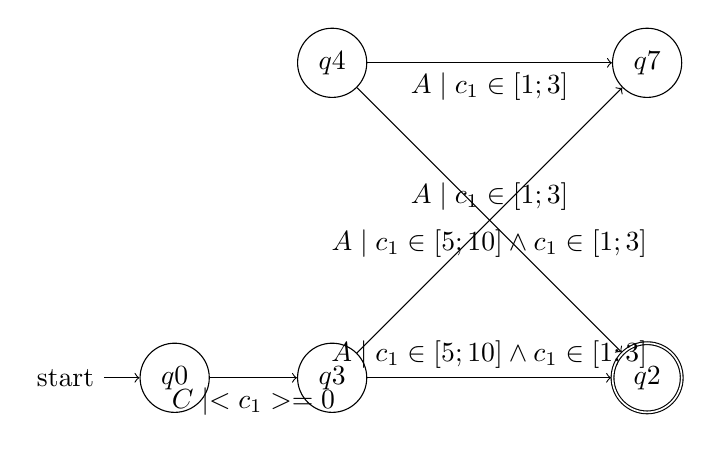
\begin{tikzpicture}[auto]
    \node[state, initial] at (0, 0)(q0){$q0$};
    \node[state] at (2, 0)(q3){$q3$};
    \node[state] at (2, 4)(q4){$q4$};
    \node[state] at (6, 4)(q7){$q7$};
    \node[state, accepting] at (6, 0)(q2){$q2$};
    
    \path[->]
        (q4)edge node[below]{$A\mid c_1\in[1;3]$}(q7)
        (q3)edge node[above]{$A\mid c_1\in[1;3]$}(q7)
        (q4)edge node[below]{$A\mid c_1\in[5;10]\wedge c_1\in[1;3]$}(q2)
        (q3)edge node[above]{$A\mid c_1\in[5;10]\wedge c_1\in[1;3]$}(q2)
        (q0)edge node[below]{$C\mid <c_1>=0$}(q3)
        ;
\end{tikzpicture}
 

\end{frame}
\begin{frame}{Dead transition}
    Pruning dead edges means pruning all edges that can never be taken because they are overconstrained.

We do this by first taking the intersection of all edges with multiple ranges.
If this intersection has no possible values we know the edge cannot possibly be taken.
Since it cannot be taken we can remove it.

Mathematically this can be described as a function ($\mathbb{E}$) taking in an automaton and returning a new automaton with the dead edges being pruned.

\sembox{
    $\deadedge(A)=\automaton[][Q][C][\Delta'][\Sigma][s][F]$
 
    $\Delta'=\{\transition\in\Delta\mid\phi\neq\emptyset\wedge\emptyset\neq\cap_{i=1}^n\phi_i\}$

}
    % Generated by: TimedRegex, Version = 1.0.0.0
% Date 5/14/2024 6:44:16 PM
\usetikzlibrary {automata,positioning}
\scalebox{0.9}{
    % "C(A[5;10]&(BA|A)[1;3])"
    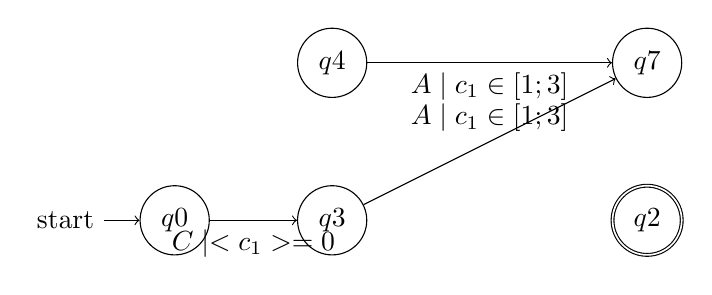
\begin{tikzpicture}[auto]
        \node[state, initial] at (0, 0)(q0){$q0$};
        \node[state] at (2, 0)(q3){$q3$};
        \node[state] at (2, 2)(q4){$q4$};
        \node[state] at (6, 2)(q7){$q7$};
        \node[state, accepting] at (6, 0)(q2){$q2$};
        
        \path[->]
            (q4)edge node[below]{$A\mid c_1\in[1;3]$}(q7)
            (q3)edge node[above]{$A\mid c_1\in[1;3]$}(q7)
            (q0)edge node[below]{$C\mid <c_1>=0$}(q3)
            ;
    \end{tikzpicture}
}

\captionof{figure}{Dead transitions $q4\rightarrow q2$ and $q3\rightarrow q2$ have been removed.}
\label{fig:prune2}

\end{frame}
\begin{frame}{Unreachable state}
    Unreachable states are very similar to dead states.
Except we check for any edges that end at a given state.
If a state is not reachable it is removed.
Repeat until no such states exist.

\sembox{
    $\unreachable(A_1)=\left\{\begin{array}{ll}
        A_1 & if \forall q_1\in Q_1:q_1'\notin F_1\wedge\transition[_1]\in\Delta_1 \\
        \unreachable(\automaton[][Q][C_1][\Delta][\Sigma_1][s_1][F_1]) & otherwise \\
    \end{array}\right.
    $

    $Q=\{q_1'\in Q_1\mid q_1\notin F_1\wedge\transition[_1]\in\Delta_1\}$

    $\Delta=\{\transition[_1]\in\Delta_1\mid q_1'\in Q\}$
}
    % Generated by: TimedRegex, Version = 1.0.0.0
% Date 5/14/2024 6:44:16 PM
\usetikzlibrary {automata,positioning}
\scalebox{0.9}{
    % "C(A[5;10]&(BA|A)[1;3])"
    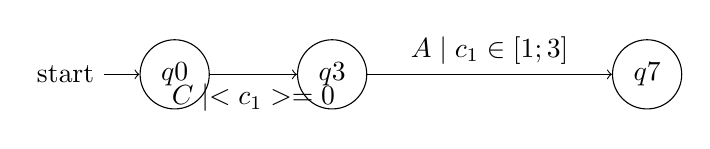
\begin{tikzpicture}[auto]
        \node[state, initial] at (0, 0)(q0){$q0$};
        \node[state] at (2, 0)(q3){$q3$};
        \node[state] at (6, 0)(q7){$q7$};
        
        \path[->]
            (q3)edge node[above]{$A\mid c_1\in[1;3]$}(q7)
            (q0)edge node[below]{$C\mid <c_1>=0$}(q3)
            ;
    \end{tikzpicture}
}

\captionof{figure}{Unreachable states $q4$ and $q2$ have been removed.}
\label{fig:prune3}

\end{frame}
\begin{frame}{Dead state}
    Dead states are all the states that have no way of reaching the final state.
These states are pruned by removing all states that have no edges away from them unless they are final states, this is repeated untill no states satisfy this property.

\sembox{
    $\deadstate(A_1)=\left\{\begin{array}{ll}
        A_1 & if \forall q_1\in Q_1:q_1\notin F_1 \transition[_1]\in\Delta_1 \\
        \deadstate(\automaton[][Q][C_1][\Delta][\Sigma_1][s_1][F_1]) & otherwise \\
    \end{array}\right.
    $

    $Q=\{q_1\in Q_1|q_1\notin F_1\wedge\transition[_1]\in\Delta_1\}$

    $\Delta=\{\transition[_1]\in\Delta_1|q_1\in Q\}$
}
    % Generated by: TimedRegex, Version = 1.0.0.0
% Date 5/14/2024 6:44:16 PM
\usetikzlibrary {automata,positioning}
% "C(A[5;10]&(BA|A)[1;3])"
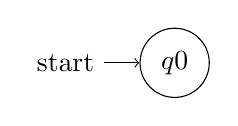
\begin{tikzpicture}[auto]
    \node[state, initial] at (0, 0)(q0){$q0$};
    
    \path[->]
        ;
\end{tikzpicture}
 

\end{frame}
\begin{frame}{Dead clock}
    % Any clocks that are not used in any intervals can be removed.
% This means removing them both from the clocks set and from any clock resets.
% This shouldn't have a huge impact, but it will allow us to create a more minimal declaration field in Uppaal.
\begin{definition}\label{definition:deadClockPruning}
    Dead clock pruning:
    \vspace{0.5em}

    \sembox{
        $\deadclock\automaton=\automaton[][Q][C'][\Delta'][\Sigma][s][F]$

        \vspace{0.5em}

        $C'=\{c\mid\exists\transition[]\in\Delta:\exists(c',I) \in\phi:c=c'\}$

        $\Delta'=\{\transition[][q][q'][\phi][p\cap C']\mid\transition\in\Delta\}$
    }
\end{definition}
    % Generated by: TimedRegex, Version = 1.0.0.0
% Date 5/14/2024 6:44:16 PM
\usetikzlibrary {automata,positioning}
% "C(A[5;10]&(BA|A)[1;3])"
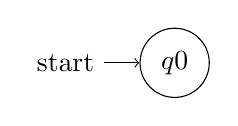
\begin{tikzpicture}[auto]
    \node[state, initial] at (0, 0)(q0){$q0$};
    
    \path[->]
        ;
\end{tikzpicture}
 

\end{frame}
\begin{frame}{Recursion}
    \begin{definition}\label{definition:recursivePruning}
    Recursive pruning:
    
    \sembox{
        $\pruning(A)=\left\{\begin{array}{ll}
            A & \text{if }A=A' \\
        \pruning(A') & otherwise \\
        \end{array}\right.
        $

        $A' = \clockreduction\circ\deadedge\circ\deadstate\circ\unreachable\circ\deadclock(A)$
    }
\end{definition}
    % Generated by: TimedRegex, Version = 1.0.0.0
% Date 5/14/2024 6:44:16 PM
\usetikzlibrary {automata,positioning}
\scalebox{0.9}{
    % "C(A[5;10]&(BA|A)[1;3])"
    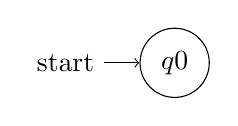
\begin{tikzpicture}[auto]
        \node[state, initial] at (0, 0)(q0){$q0$};
    \end{tikzpicture}
}

\captionof{figure}{Final pruned automaton.}
\label{fig:prune6}

\end{frame}

\begin{frame}
    \begin{definition}\label{definition:recursivePruning}
    Recursive pruning:
    
    \sembox{
        $\pruning(A)=\left\{\begin{array}{ll}
            A & \text{if }A=A' \\
        \pruning(A') & otherwise \\
        \end{array}\right.
        $

        $A' = \clockreduction\circ\deadedge\circ\deadstate\circ\unreachable\circ\deadclock(A)$
    }
\end{definition}
    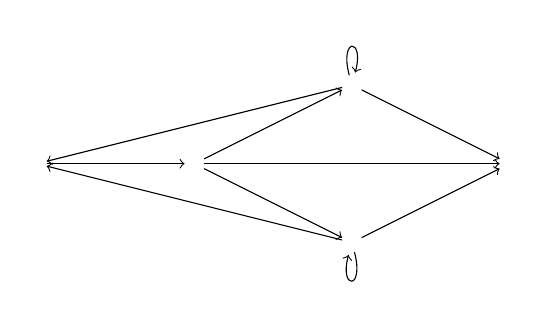
\begin{tikzpicture}[auto]
    \node[] at (0, 0)(cr){$\clockreduction$};
    \node[] at (4, -1)(sd){$\deadstate$};
    \node[] at (4, 1)(su){$\unreachable$};
    \node[] at (2, 0)(td){$\deadedge$};
    \node[] at (6, 0)(cd){$\deadclock$};
    
    \path[->]
        (su)edge [loop above] node{}(su)
        (sd)edge [loop below] node{}(sd)
        (su)edge node[align=left]{}(cr)
        (sd)edge node[align=left]{}(cr)
        (td)edge node[align=left]{}(sd)
        (td)edge node[align=left]{}(su)
        (sd)edge node[align=left]{}(cd)
        (su)edge node[align=left]{}(cd)
        (td)edge node[align=left]{}(cd)
        (cr)edge node[align=left]{}(td)
        ;
\end{tikzpicture}
\end{frame}

% =======================================================================
% Graph layout
% =======================================================================
\section{Graph layout}
\begin{frame}
    We dont need precise algorithm
    \begin{itemize}
        \item Make graph acyclic (trivial)
        \item Assign states to layers
        \item Order states in layers (just needs to be good enough)
        \item Assign positions (simplicity over correctness)
    \end{itemize}
\end{frame}

\begin{frame}[fragile]{Creation of recursive edges}
    In automaton generator visitor
    \begin{lstlisting}[language=c++,basicstyle=\tiny]
public void Visit(GuaranteedIterator guaranteedIterator)
{
    TimedAutomaton ta = _stack.Pop();

    foreach (Edge oldEdge in ta.GetEdgesTo(ta.GetFinalStates()).ToList())
    {
        Edge edge = ta.AddEdge(oldEdge.From, ta.InitialState!, oldEdge.Symbol, true);
        edge.AddClockRanges(oldEdge.GetClockRanges());
        edge.AddClockResets(ta.GetClocks());
    }

    _stack.Push(ta);
}
    \end{lstlisting}
    \begin{lstlisting}[language=c++,basicstyle=\tiny]
public void Visit(AbsorbedGuaranteedIterator absorbedGuaranteedIterator)
    ...
    foreach (Edge childEdge in child.GetEdges())
        ...
        foreach (SortedSet<Clock> clockSet in clockPowerSet)
            ...    
            if (child.IsFinal(childEdge.To))
            {
                edge = ta.AddEdge(from, ta.InitialState!, childEdge.Symbol, true);
                edge.AddClockResets(childEdge.GetClockResets());
                edge.AddClockRanges(ranges);
            }
            ...
        ...
    ...
    \end{lstlisting}
\end{frame}

\begin{frame}[fragile]{Keeping reversible edges}
    In automaton generator visitor
    \begin{lstlisting}[language=c++,basicstyle=\tiny]
public void Visit(AbsorbedGuaranteedIterator absorbedGuaranteedIterator)
...
foreach (Edge childEdge in child.GetEdges())
    ...
    foreach (SortedSet<Clock> clockSet in clockPowerSet)
        ...
        Edge edge = ta.AddEdge(from, to, childEdge.Symbol, childEdge.IsReversible);
        edge.AddClockResets(childEdge.GetClockResets());
        edge.AddClockRanges(ranges);
        ...
    ...
...
    \end{lstlisting}
    
    \begin{lstlisting}[language=c++,basicstyle=\tiny]
public void Visit(Intersection intersection)
...
foreach (Edge lEdge in lEdges)
    ...
    foreach (Edge rEdge in rEdges)
        ...
        State from = GetNewEdge(lEdge.From, rEdge.From);
        State to = GetNewEdge(lEdge.To, rEdge.To);
        Edge edge = ta.AddEdge(from, to, c, lEdge.IsReversible || rEdge.IsReversible);
        edge.AddClockRanges(lEdge.GetClockRanges().Concat(rEdge.GetClockRanges()));
        edge.AddClockResets(lEdge.GetClockResets().Concat(rEdge.GetClockResets()));
        ...
    ...
...
    \end{lstlisting}
\end{frame}

\begin{frame}[fragile]{Removing recursive edges}
    In graphlayout
    \begin{lstlisting}[language=c++,basicstyle=\tiny]
private void AssignLayers(TimedAutomaton ta, TaState taState, int layerIndex)
...
foreach (Edge edge in ta.GetEdgesFrom(taState)
    .Where(e => !e.IsReversible))
    ...
foreach (Edge edge in ta.GetEdgesTo(taState)
    .Where(e => e.IsReversible && !e.To.Equals(taState)))
    ...
...
    \end{lstlisting}
\end{frame}